\documentclass{article}
\usepackage[preprint]{neurips_2026}
\usepackage[T1]{fontenc}
\usepackage{microtype,xcolor}
\usepackage{amsmath,amssymb,amsthm,graphicx,booktabs}
\usepackage[hidelinks]{hyperref}
\newtheorem{theorem}{Theorem}
\newtheorem{proposition}[theorem]{Proposition}
\newtheorem{corollary}[theorem]{Corollary}
\newtheorem{lemma}[theorem]{Lemma}
\newcommand{\E}{\mathbb E}
\newcommand{\Pp}{\mathbb P}
\newcommand{\ind}{\mathbf 1}
\title{Joint Risk and Review-Budget Certification for Consent-Constrained Incident Alerts}
\author{Aravind Kannappan}
\date{October 2026}
\begin{document}
\maketitle
\begin{abstract}
Clinical monitoring must reconcile timely event detection, patient consent and finite review capacity. We show that allowing only the first threshold crossing can make incident missed-event loss non-monotone: a lower threshold may consume the review before the valid warning window. We characterize the minimum feasible review budget using pre-window and in-window score maxima, and apply simultaneous binomial bounds to distinguish certified feasibility, grid infeasibility and insufficient evidence. We also state when consent transformations preserve the sampling assumptions and give a counterexample under consent-mechanism shift. An evaluation on all 40,336 public PhysioNet 2019 patients compares tuned logistic regression, gradient boosting and a GRU across three seeds and two hospitals. Mean pre-onset AUROC reaches 0.794 at hospital A and 0.752 externally. Yet every locally calibrated first-alert grid is excluded at a 5\% conditional missed-event target, even with one review per patient. Positive challenge utility does not resolve this failure because it rewards a different warning window and persistent prediction state. Patient-specific consent and reviewer simulations extend the evaluation but do not establish clinical effectiveness. The study identifies a policy-level obstacle that better score discrimination alone does not remove.
\end{abstract}

\section{Question and contribution}
The motivating question is whether a clinical monitoring pipeline can retain useful predictions while its data flows, model errors, and consequential decisions are governed by explicit consent and effective human oversight. This conjunction requires more than a structural graph check or a discrimination score. We separate (i) compliance of a specified information graph, (ii) statistical error and workload of an alert policy, and (iii) timely and correct action by human reviewers.

Our technical development concerns the second component. The main distinction is between nested threshold \emph{crossings} and timely \emph{first alerts}. Their losses need not share monotonicity. We derive a score-distribution feasibility characterization and implement joint confidence certification for a validation-frozen finite grid. The underlying confidence machinery follows Learn then Test (LTT) and risk-controlling prediction sets \citep{ltt,rcps}; simultaneous risk/cost optimization is also studied by Pareto Testing \citep{pareto}. We do not claim to invent these frameworks. The proposed contribution is their careful application to consent-dependent incident alerts, the first-alert failure mode, and an auditable clinical evaluation. Recent clinical selective-prediction work combines conformal prediction with cost-aware deferral \citep{kwon2026}. Here the unit of risk is a missed incident event, and the unit of capacity is a patient review; prediction-set coverage and error on retained cases answer different questions.

\section{Setup and incident policies}
A patient supplies a finite sequence of causally available observations, consent states, and frozen scores $S_1,\ldots,S_T\in[0,1]$. Let $Z$ indicate an incident event with an observed valid warning window $[a,b]$. For a threshold $\tau$, the first-alert policy is
\begin{equation}
 T_\tau=\inf\{t:S_t\ge\tau\},\qquad
 R_\tau=\ind\{T_\tau\le T\},\qquad
 L_\tau=\ind\{T_\tau\notin[a,b]\},\quad Z=1.
 \label{eq:first}
\end{equation}
An empty set gives $T_\tau=\infty$. Assume $0<\Pr(Z=1)<1$ and $0<\alpha<1$. We target conditional incident risk $r(\tau)=\E[L_\tau\mid Z=1]$ and expected workload $w(\tau)=\E[R_\tau]$, measured in reviews per patient. Their joint constraints are $r(\tau)\le\alpha$ and $w(\tau)\le K$. For $m$ independent patient arrivals in a period, the expected number of reviews is $mw(\tau)$; an expectation bound does not guarantee a finite waiting time.

For comparison, a repeated-alert policy uses every threshold crossing. Its incident missed-event loss is $\ind\{\max_{a\le t\le b}S_t<\tau\}$, which is monotone in $\tau$. A rule that emits only the first crossing has lower review count but a different risk.

\begin{proposition}[First-alert non-monotonicity]\label{prop:nonmono}
Nested threshold crossings do not imply monotone timely first-alert loss. There is a trajectory for which lowering $\tau$ changes the incident loss from zero to one, although the probability of any review is non-decreasing as the threshold decreases.
\end{proposition}
\begin{proof}
Let a pre-window score equal $0.6$, an in-window score equal $0.9$, and all other scores equal zero. At threshold $0.8$, the first alert lies inside the window and loss is zero. At threshold $0.5$, the first alert occurs before the window and consumes the only alert; loss is one. Both thresholds trigger exactly one review. A threshold above $0.9$ yields no alert and loss one. Thus the loss sequence as thresholds increase is $1,0,1$. Any-review events remain nested because they depend only on the overall score maximum.
\end{proof}
This prevents applying the monotone-loss conformal risk-control theorem \citep{crc} to the first-alert loss without additional assumptions. Counting any in-window crossing while reporting only one early review would evaluate a different policy.

\section{Population feasibility}
Define the pre-window maximum $A=\max_{t<a}S_t$, with $A=-\infty$ for an empty prefix, the in-window maximum $B=\max_{a\le t\le b}S_t$, and the maximum $C$ over the monitoring interval used to count reviews. For event-positive patients the monitoring interval includes the warning window. Let $\pi=\Pp(Z=1)$ and
\begin{equation}
 H(\tau)=\Pp(A<\tau\le B\mid Z=1),\qquad
 W(\tau)=\pi\Pp(C\ge\tau\mid Z=1)+(1-\pi)\Pp(C\ge\tau\mid Z=0).
 \label{eq:HW}
\end{equation}

\begin{theorem}[Exact feasibility of a first-alert threshold family]\label{thm:feas}
For a fixed threshold domain $\mathcal T$, a jointly feasible first-alert threshold exists if and only if
\[
 \{\tau\in\mathcal T:H(\tau)\ge 1-\alpha,\ W(\tau)\le K\}\ne\varnothing.
\]
If $\mathcal T_\alpha=\{\tau\in\mathcal T:H(\tau)\ge1-\alpha\}$ is nonempty and has a maximum $\tau_\star$, the minimum feasible expected review budget is
\begin{equation}
 K_{\min}=W(\tau_\star).
 \label{eq:kmin}
\end{equation}
Consequently, joint feasibility is equivalent to $K\ge K_{\min}$. Moreover $K_{\min}\ge\pi(1-\alpha)$. If $\mathcal T_\alpha$ is empty, no review budget makes this threshold family feasible.
\end{theorem}
The maximum assumption always holds for a finite nonempty policy grid. For a continuous domain it is a substantive attainment condition; replacing a minimum by an infimum without attainment can make a boundary feasibility assertion false. This characterization is exact but needs the joint law of $A$ and $B$, not merely an hourly ROC curve.

\begin{corollary}[Closed form when early consumption is absent]\label{cor:quantile}
Suppose no alert is possible before the valid window, the positive-patient review interval equals that window, and the conditional distributions of $C$ are continuous, with positive-class CDF $F_1$ strictly increasing at its unique $\alpha$-quantile $q_\alpha$. Let the negative-class CDF be $F_0$. Then
\begin{equation}
 K_{\min}=\pi(1-\alpha)+(1-\pi)\{1-F_0(q_\alpha)\},\qquad q_\alpha=F_1^{-1}(\alpha).
\end{equation}
This is the familiar threshold/ROC workload identity under an explicit no-early-consumption assumption; it is not a general formula for an unrestricted first-alert policy.
\end{corollary}

\section{Finite-sample joint certification}
Let $\mathcal T=\{\tau_1,\ldots,\tau_M\}$ be fixed independently of calibration data, for example using training and validation only. Calibration patients are independent and identically distributed from the deployment population, including the consent mechanism. For each policy compute positive-patient losses and all-patient review indicators. Let $n_+$ be the positive calibration count and $n$ the total count. Use exact one-sided Clopper--Pearson binomial bounds with tail probability $\eta=\delta/(4M)$ to obtain $(\ell^r_j,u^r_j)$ and $(\ell^w_j,u^w_j)$.

\begin{theorem}[Joint certificate and honest abstention]\label{thm:certificate}
Conditional on any independently trained predictor and frozen grid, with probability at least $1-\delta$ over calibration, all of the following hold simultaneously:
\begin{enumerate}
\item Every $j$ with $u^r_j\le\alpha$ and $u^w_j\le K$ satisfies both population constraints.
\item If every $j$ has $\ell^r_j>\alpha$ or $\ell^w_j>K$, no policy on this grid satisfies both constraints.
\item Any data-dependent selection among certified policies, including the one with smallest workload upper bound, preserves assertion 1.
\end{enumerate}
No monotonicity of $L_\tau$ is required. If neither condition 1 nor condition 2 is met, the output is \emph{undetermined}, not infeasible. For $n_+=0$, the risk interval is $[0,1]$ and no positive-risk claim is certified.
\end{theorem}
The construction applies simultaneous-confidence/LTT reasoning to the first-alert policy in Proposition~\ref{prop:nonmono}. The three outputs distinguish an acceptable operating point, an excluded grid, and a calibration sample that cannot resolve the question.

The certificate is a high-probability statement about the population risk of the selected policy, distinct from the expectation-over-calibration guarantee of ordinary CRC. Model selection performed on calibration would require including every candidate model/policy in the multiplicity family; here model tuning uses validation only. Separate per-model certificates are not automatically simultaneous across models or seeds.

\begin{corollary}[Prespecified group or site cells]
For groups $g=1,\ldots,G$ specified independently of calibration, apply Theorem~\ref{thm:certificate} within each cell using $\delta_g$ with $\sum_g\delta_g\le\delta$. All certified group-conditional risk and workload statements then hold jointly with probability at least $1-\delta$. The groups may overlap. Empty or underpowered cells can remain undetermined. A rule calibrated in one hospital is not certified in another merely by relabeling its population.
\end{corollary}

\section{Consent, exchangeability and shift}
Let $U$ denote the complete patient trajectory, $C$ the possibly time-varying consent trajectory, and $V$ any policy randomization. A frozen causal procedure $\Phi(U,C,V)$ produces permitted features, scores, alert decisions, and losses. The procedure may clear cached features and recurrent state after revocation.

\begin{proposition}[Sufficient exchangeability condition]\label{prop:consent}
If the calibration and future tuples $(U,C,V)$ are identically distributed and independent, and the same frozen measurable transformation $\Phi$ is applied to every tuple, their loss and review vectors are identically distributed and independent. Theorem~\ref{thm:certificate} therefore remains valid, including after conditioning on positive-event membership. Consent need not be independent of the outcome.
\end{proposition}
The weaker condition $C\perp Y\mid X$ alone does not guarantee transfer between different consent populations. For a counterexample, let $X=Y\sim\mathrm{Bernoulli}(1/2)$ and score $S=CX$. Calibration consent is always $C=1$, deployment consent always $C=0$, and the threshold is $1/2$. Both populations satisfy $C\perp Y\mid X$, yet positive-patient missed risk changes from zero to one. Conditional ignorability does not make the joint distributions equal.

\begin{theorem}[Known-ratio shift certificate]\label{thm:weighted}
Suppose the target patient law $Q$ is absolutely continuous with respect to source law $P$, with known density ratio $0\le w\le B_w$ and $\E_Pw=1$. For a fixed grid and $n$ independent source patients define
\[
 \widehat a_j=n^{-1}\sum_i w_iZ_iL_{ij},\quad
 \widehat b=n^{-1}\sum_i w_iZ_i,\quad
 \widehat c_j=n^{-1}\sum_i w_iR_{ij}.
\]
Set $\epsilon=B_w\sqrt{\log((2M+1)/\delta)/(2n)}$.
With probability at least $1-\delta$, simultaneously for every $j$ with $\widehat b>\epsilon$,
\[
 \E_Q[L_j\mid Z=1]\le\min\left\{1,\frac{\widehat a_j+\epsilon}{\widehat b-\epsilon}\right\},\qquad
 \E_Q[R_j]\le\min\{1,\widehat c_j+\epsilon\}.
\]
Thus selecting a policy whose two upper bounds meet $(\alpha,K)$ controls both target quantities. If the denominator is nonpositive, the risk bound is uninformative.
\end{theorem}
This is a bounded-importance-weight Hoeffding argument. A feature-only density ratio is valid only under the corresponding conditional outcome invariance and support assumptions. A fitted, clipped domain classifier does not provide a known ratio or a verified bound on approximation error. Our empirical weighted comparison is explicitly exploratory, not an application of Theorem~\ref{thm:weighted} with a guaranteed ratio.

\section{Empirical protocol}
\paragraph{Data and endpoint.} We use all 20,336 hospital-A and 20,000 hospital-B patient files from the public PhysioNet/CinC 2019 release \citep{physionet}. Published labels already start six hours before inferred onset. We do not shift them again. The primary incident window starts at the first positive label and ends immediately before inferred onset. Initial-positive patients and patients whose inferred onset is outside the observed stay are excluded from conditional incident risk but retained in workload. Reviews are counted before inferred onset in positive patients and over the observed stay in negative patients. This outcome-defined stopping rule is retrospective; deployment would need an observable stopping mechanism. The warning window is stricter than the challenge utility window.

\paragraph{Splits and models.} Each of three seeds splits A 55/15/15/15\% into training, validation, calibration, and test. B reserves 25\% for local calibration and keeps 75\% as a frozen external test. Logistic regression tunes regularization and class weighting; histogram gradient boosting tunes tree size, regularization and weighting; a unidirectional GRU tunes hidden size and validation-selected epoch under a fixed six-epoch budget. Training loss and primary discrimination exclude post-onset rows. Every preprocessing fit uses training data only. Model selection uses validation average precision. Causal tests perturb later observations and verify unchanged earlier features.

\paragraph{Policies and uncertainty.} Candidate score thresholds are quantiles frozen on validation data. We compare repeated crossings with first alerts and report conditional incident missed-event risk, reviews per patient, and the official challenge utility. The latter evaluates full-stay predicted condition states; for once-only review we report a latched positive state after the first alarm, rather than pretend a single positive hour represents all subsequent clinical knowledge. It is a distinct metric. All seeds receive 500 patient-cluster bootstrap replicates. Repeated calibration subsets quantify stability but overlap; their empirical exceedance fractions are not independent clinical trials.

\paragraph{Consent and reviewer process.} Patient-specific opt-outs of labs and vitals are simulated at rates 0, .1, .3 and .5. Separate revocation scenarios apply at hour 12, remove prohibited historical summaries and clear recurrent state. The model is frozen; these stress tests do not claim to infer actual consent preferences. Queue arrivals use sepsis prediction trajectories, with service-time, sensitivity, specificity and fatigue sweeps. Timing of actual clinical response is distinct from active review service time: published TREWS adoption work reports provider response windows \citep{trews}, but does not justify treating a two-, five-, or ten-minute service time as an empirically measured constant. Our service and arrival parameters remain sensitivity assumptions. Five hundred random pipeline DAGs supplement the fixed information graph; neither is a deployed-system audit.

\section{Results and scope}
\paragraph{Stronger discrimination does not settle alert feasibility.}
Table~\ref{tab:discrimination} summarizes all three splits. Boosting has the highest mean AUROC in A; the GRU has the highest mean AUROC in B. These are descriptive rankings: the seed-specific test populations overlap. Average precision remains low, and the class-weighted models are not calibrated probabilities. Full patient-bootstrap intervals and Brier scores are in the appendix.
\begin{table}[t]
\centering
\caption{Pre-onset discrimination, mean across three seeds. AP denotes average precision. Per-seed 95\% patient-bootstrap intervals appear in Table~\ref{tab:allseeds}; seed averaging is not an independent-cohort meta-analysis.}
\label{tab:discrimination}
\begin{tabular}{lrrrr}\toprule
Model & AUROC A & AUROC B & AP A & AP B\\\midrule
Logistic & 0.745 & 0.666 & 0.049 & 0.025 \\
Boosting & 0.794 & 0.731 & 0.060 & 0.033 \\
GRU & 0.778 & 0.752 & 0.060 & 0.031 \\
\bottomrule\end{tabular}\end{table}

\paragraph{The first-alert target is not achieved.}
For every model and seed, the local A and B calibrations certify grid infeasibility at $\alpha=0.05$, for every tested budget from 0.1 to 1 review per patient. There are 90 local calibration/budget outcomes; each certificate retains its stated per-grid confidence interpretation. The result concerns the frozen grids, not all thresholds or all monitoring designs. Increasing review capacity cannot repair a grid whose first-alert timing already violates the risk target.

\begin{figure}[t]
\centering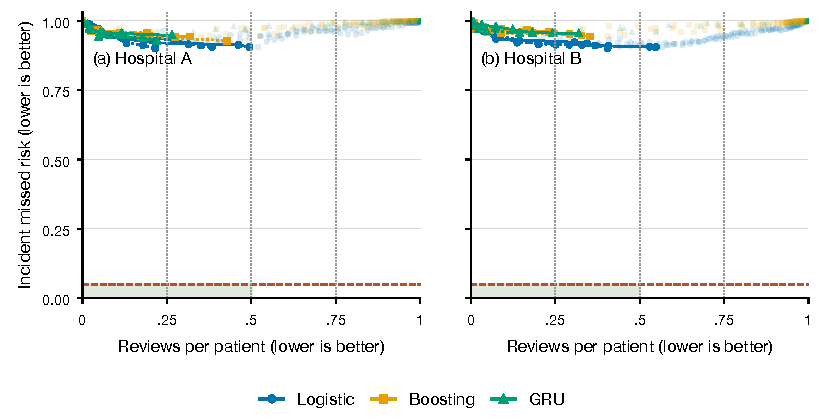
\includegraphics[width=\linewidth]{figs/incident_frontier.pdf}
\caption{\textbf{The tested first-alert grids remain far from the target region.} All three seeds are shown (solid, dashed and dotted), with faint markers for dominated thresholds. Each model has 51 validation-quantile candidates plus endpoints before deduplication. Lines are frontier guides, not attainable interpolations. Shading marks risk $\le0.05$ and workload $\le0.5$. Panels show hospitals A and B.}
\label{fig:frontier}
\end{figure}

Figure~\ref{fig:frontier} also shows the realized test risks. Even the best test-grid point, selected retrospectively only to describe the frontier, misses at least 90.0\% of eligible incidents. This stringent endpoint treats a review just before the six-hour window as a miss, even if it might be useful clinically. The negative result is therefore about timely \emph{first} review under this definition, not about whether early alerts have clinical value.

\paragraph{Policy choice explains the apparent contradiction with utility.}
We additionally choose thresholds by validation challenge utility and freeze them before testing (Table~\ref{tab:policies}). Boosting in A achieves mean utility 0.332 with 0.193 reviews per patient, yet its strict incident missed risk is 0.960. Its three test splits contain 742 eligible incident observations in total, counting overlap across splits: 414 receive an early first alert and 298 receive none before onset. Only 30 receive their first alert in the specified window. The challenge utility credits a broader time window and a persistent positive state; it is not a surrogate for this first-review endpoint.

Repeated alerts recover more incidents but require several reviews per patient. At validation-selected utility thresholds, no model/site/policy combination has all three of positive utility, risk at most 0.05, and workload at most 0.5. This is the empirical answer to the declared joint target, not proof against alternative cooldown or continuing-review policies.
\begin{table}[t]
\centering\small
\caption{Validation-selected operating policies, means over three seeds. ``Repeated'' reviews every above-threshold hour. Utility uses full-stay states; risk and review count use the retrospective pre-onset endpoint. No test metric chooses a threshold.}
\label{tab:policies}
\begin{tabular}{lllrrr}\toprule
Model & Site & Policy & Missed risk & Reviews/patient & Utility\\\midrule
Logistic & A & First & 0.936 & 0.215 & 0.333 \\
Logistic & A & Repeated & 0.298 & 8.077 & 0.342 \\
Logistic & B & First & 0.916 & 0.296 & 0.085 \\
Logistic & B & Repeated & 0.302 & 10.185 & 0.003 \\
Boosting & A & First & 0.960 & 0.193 & 0.332 \\
Boosting & A & Repeated & 0.318 & 6.741 & 0.380 \\
Boosting & B & First & 0.970 & 0.091 & 0.125 \\
Boosting & B & Repeated & 0.494 & 4.162 & 0.183 \\
GRU & A & First & 0.949 & 0.160 & 0.347 \\
GRU & A & Repeated & 0.406 & 6.124 & 0.352 \\
GRU & B & First & 0.971 & 0.081 & 0.155 \\
GRU & B & Repeated & 0.534 & 4.172 & 0.180 \\
\bottomrule\end{tabular}\end{table}

\paragraph{Recalibration, consent and review.}
Local B calibration contains 230--242 eligible positives, compared with 219--253 in A. None of 14,400 overlapping calibration subsets (25, 50, 100 or 200 positives) certifies the 5\% first-alert risk target. Thus the fraction of test-risk violations \emph{among certified rules} is undefined, not zero. Four hundred positives are unavailable in these calibration pools; the study does not establish how much additional data would suffice. All 72 prespecified group/model/site/seed checks also exclude their tested grids.

Consent interventions do not restore feasibility. They change both scores and the descriptive fallback threshold, so a reduced review count need not be an improvement. For example, GRU opt-out at 50\% per feature group changes mean A missed risk from 0.952 to 0.979 while reviews fall from 0.207 to 0.104 per patient. These are simulated permissions, not observed patient preferences. The estimated-ratio repeated-alert diagnostic has external-site risk from 0.034 to 0.152 across model/seed combinations and carries no exact shift guarantee.

The corrected reviewer audit evaluates 972 queue scenarios on frozen scores. Across all these scenarios, end-to-end missed risk ranges from 0.912 to 0.987; a perfect reviewer cannot recover an incident that never receives a timely review. The simulation is not evidence about real clinician performance. Among 500 random DAGs, 126 contain a source-to-action path and 103 contain a path bypassing the randomly assigned review nodes. This illustrates why review nodes alone do not enforce review, while remaining a synthetic structural test.



The earlier 6,000-patient hourly-alert study is retained as historical supplementary evidence. The small MIMIC demo and five-participant movement track are excluded from the revised primary analysis. Full credentialed MIMIC-IV has not been evaluated. A benchmark row satisfying empirical utility, risk, workload and structural constraints does not establish actual clinician competence or patient benefit.

\section{Discussion}
The answer to the motivating question is conditional. We can specify consent constraints, verify mandatory review paths and evaluate statistical risk against capacity. The evaluated first-alert pipelines do not meet the declared incident-risk target, despite positive challenge utility. This supplies a concrete negative answer for the tested family; it leaves the broader design question open.

A mathematical certificate must cover the policy actually deployed. Restricting review count can change the shape of incident risk, so a throughput improvement cannot be assumed to preserve a monotone CRC theorem. Our three-way certification outcome prevents a failed bound from being mislabeled as an impossibility result. A successful certificate establishes a retrospective distributional property under explicit sampling assumptions; prospective care effectiveness remains a separate empirical question. A practical follow-up should evaluate cooldown and continuing-review policies that retain the value of an early assessment. Those policies need their own workload definition and certificate; they cannot inherit the first-alert result automatically.

The principal limitations are a strict retrospective warning window, a finite threshold grid, modest tuning budgets, overlapping seed splits, simulated consent and assumed reviewer parameters. We study two public hospitals, not prospective care. Consent masks are not a complete privacy or security mechanism, and a mandatory graph node does not establish that a clinician understands or acts on an alert. Deploying these prototypes as if those properties had been established would create false reassurance and avoidable review burden.

\begin{thebibliography}{9}
\bibitem[Kwon and Kim(2026)]{kwon2026} H. Kwon and D.-J. Kim. Conformal selective prediction with cost aware deferral for safe clinical triage under distribution shift. Scientific Reports, 16:10016, 2026. \url{https://doi.org/10.1038/s41598-026-40637-w}.
\bibitem[Angelopoulos et al.(2024)]{crc} A. N. Angelopoulos, S. Bates, A. Fisch, L. Lei, and T. Schuster. Conformal Risk Control. ICLR, 2024. \url{https://arxiv.org/abs/2208.02814}.
\bibitem[Angelopoulos et al.(2025)]{ltt} A. N. Angelopoulos, S. Bates, E. J. Cand\`es, M. I. Jordan, and L. Lei. Learn then test: Calibrating predictive algorithms to achieve risk control. Annals of Applied Statistics, 2025. \url{https://doi.org/10.1214/24-aoas1998}.
\bibitem[Bates et al.(2021)]{rcps} S. Bates, A. N. Angelopoulos, L. Lei, J. Malik, and M. I. Jordan. Distribution-free, risk-controlling prediction sets. Journal of the ACM, 2021. \url{https://doi.org/10.1145/3478535}.
\bibitem[Laufer-Goldshtein et al.(2023)]{pareto} B. Laufer-Goldshtein, A. Fisch, R. Barzilay, and T. Jaakkola. Efficiently Controlling Multiple Risks with Pareto Testing. ICLR, 2023. \url{https://arxiv.org/abs/2210.07913}.
\bibitem[Reyna et al.(2019)]{physionet} M. A. Reyna et al. Early Prediction of Sepsis from Clinical Data: The PhysioNet/Computing in Cardiology Challenge 2019, version 1.0.0. \url{https://doi.org/10.13026/v64v-d857}.
\bibitem[Henry et al.(2022)]{trews} K. E. Henry et al. Factors driving provider adoption of the TREWS machine learning-based early warning system and its effects on sepsis treatment timing. Nature Medicine, 2022. \url{https://doi.org/10.1038/s41591-022-01895-z}.
\end{thebibliography}
\clearpage
\appendix
\section{Proof of population feasibility}
\begin{proof}[Proof of Theorem~\ref{thm:feas}]
A first alert is in the warning window exactly when no earlier score reaches threshold and some in-window score does. With inclusive alert ties, those events are $A<\tau$ and $B\ge\tau$. Thus $r(\tau)=1-H(\tau)$. Any review occurs exactly when $C\ge\tau$, giving $w(\tau)=W(\tau)$ by conditioning on $Z$. This proves the set characterization. The function $W$ is non-increasing in $\tau$, regardless of whether $H$ is monotone. If the risk-feasible set has maximum $\tau_\star$, its workload is no larger than at every other risk-feasible threshold, proving Equation~\eqref{eq:kmin} and both directions of the budget equivalence. Timely success implies a review, so for every risk-feasible threshold $W(\tau)\ge\Pp(Z=1,T_\tau\in[a,b])=\pi H(\tau)\ge\pi(1-\alpha)$. If the risk-feasible set is empty, increasing workload cannot create a member of it.
\end{proof}
\begin{proof}[Proof of Corollary~\ref{cor:quantile}]
With no possible earlier alert and $B=C$ on positives, $r(\tau)=\Pp(C<\tau\mid Z=1)=F_1(\tau)$ by continuity. The unique maximal feasible threshold is $q_\alpha$ under the stated strictness and attainment assumptions. Substitution into Equation~\eqref{eq:HW} gives $\pi\{1-F_1(q_\alpha)\}+(1-\pi)\{1-F_0(q_\alpha)\}$, and $F_1(q_\alpha)=\alpha$ completes the result.
\end{proof}

\section{Proof of finite-sample certification}
\begin{proof}[Proof of Theorem~\ref{thm:certificate}]
Condition on the fitted predictor and independently chosen candidate grid. For each policy, positive-patient losses are Bernoulli with mean $r_j$, conditional on the calibration positive count and membership; all-patient review indicators are Bernoulli with mean $w_j$. Inverting the binomial tails gives each one-sided interval coverage at least $1-\eta$. This remains true unconditionally by averaging over the random positive count. Dependence between policies, or between risk and workload statistics, does not affect a union bound. There are $4M$ one-sided bounds, so all cover simultaneously with probability at least $1-4M\eta=1-\delta$. On this event, upper-bound feasibility implies true feasibility for every accepted policy, hence for any selection among them. If every policy has a lower bound violating at least one constraint, each policy violates that population constraint; therefore none on the grid is feasible. If neither condition is satisfied, the intervals do not resolve the question. The $[0,1]$ convention at zero positives makes no unsupported claim.
\end{proof}
\begin{proof}[Proof of the group corollary]
Apply the preceding coverage event within each prespecified group with error probability $\delta_g$. A union bound over groups gives failure probability at most $\sum_g\delta_g$. Groups need not be independent. The conditional sampling assumptions must hold within each group, and post-hoc group discovery is not covered.
\end{proof}

\section{Proofs under consent and shift}
\begin{proof}[Proof of Proposition~\ref{prop:consent}]
For measurable sets $B_1,\ldots,B_n$, independence of the input tuples gives
$\Pp(\Phi(U_i,C_i,V_i)\in B_i,\ i=1,\ldots,n)=\prod_i\Pp((U_i,C_i,V_i)\in\Phi^{-1}(B_i))$.
Identical input laws and the same transformation give identical output laws. Conditioning independent patient tuples on their own positive-event indicators preserves the corresponding conditional product law. Nothing in the argument requires consent to be outcome-independent; it requires the complete joint patient/consent mechanism to be stable across calibration and future data.
\end{proof}
\begin{proof}[Proof of Theorem~\ref{thm:weighted}]
The random variables $wZL_j,wZ,wR_j$ all lie in $[0,B_w]$. One-sided Hoeffding bounds with failure probability $\delta/(2M+1)$ control the $M$ numerator upper deviations, one denominator lower deviation, and $M$ workload upper deviations. A union bound yields their simultaneous coverage. Change of measure gives $\E_P[wZL_j]=\E_Q[ZL_j]$, $\E_P[wZ]=\Pp_Q(Z=1)$, and $\E_P[wR_j]=\E_Q[R_j]$. When the denominator lower bound is positive, dividing its numerator upper bound by that lower bound bounds the target conditional risk. Truncation at one uses the Bernoulli range. The same simultaneous event covers data-dependent selection among accepted candidates.
\end{proof}

\section{Seed-specific uncertainty and feasibility}
\begin{table*}[t]\centering\small
\caption{All-seed pre-onset AUROC with 95\% percentile intervals from 500 whole-patient bootstrap replicates. Brier scores are point estimates; their intervals are released in the machine-readable metrics table. Intervals describe patient-sampling uncertainty conditional on each fitted model.}
\label{tab:allseeds}
\begin{tabular}{llrrrr}\toprule
Model & Seed & AUROC A [95\% CI] & AUROC B [95\% CI] & Brier A & Brier B\\\midrule
Logistic & 11 & 0.750 [0.724, 0.776] & 0.651 [0.634, 0.669] & 0.015 & 0.014 \\
Logistic & 29 & 0.738 [0.711, 0.766] & 0.679 [0.661, 0.695] & 0.187 & 0.235 \\
Logistic & 47 & 0.746 [0.718, 0.773] & 0.667 [0.649, 0.682] & 0.189 & 0.210 \\
Boosting & 11 & 0.792 [0.769, 0.818] & 0.713 [0.696, 0.732] & 0.098 & 0.060 \\
Boosting & 29 & 0.799 [0.775, 0.821] & 0.731 [0.715, 0.746] & 0.092 & 0.055 \\
Boosting & 47 & 0.792 [0.767, 0.816] & 0.748 [0.730, 0.763] & 0.014 & 0.009 \\
GRU & 11 & 0.789 [0.766, 0.816] & 0.742 [0.726, 0.759] & 0.056 & 0.043 \\
GRU & 29 & 0.787 [0.761, 0.813] & 0.752 [0.737, 0.766] & 0.057 & 0.036 \\
GRU & 47 & 0.756 [0.732, 0.782] & 0.763 [0.749, 0.777] & 0.066 & 0.053 \\
\bottomrule\end{tabular}\end{table*}


\begin{table*}[t]\centering\small
\caption{Feasibility of the validation-selected first-alert policy under conditional incident loss. Each row aggregates three seeds: ``Y'' means every seed meets the empirical criterion; ``N'' means none does. Storage and review checks concern the specified graph, not a deployed system. Actual human oversight was not measured.}
\label{tab:feasible}
\begin{tabular}{llccccc}\toprule
Model & Site & Utility $>0$ & Risk $\le .05$ & Reviews $\le .5$ & Storage cut & Review path\\\midrule
Logistic & A & Y & N & Y & Modeled & Modeled \\
Logistic & B & Y & N & Y & Modeled & Modeled \\
Boosting & A & Y & N & Y & Modeled & Modeled \\
Boosting & B & Y & N & Y & Modeled & Modeled \\
GRU & A & Y & N & Y & Modeled & Modeled \\
GRU & B & Y & N & Y & Modeled & Modeled \\
\bottomrule\end{tabular}\end{table*}


\subsection{Fixed-policy risk intervals.}
The policy audit reports 36 validation-selected operating points with exact pointwise 95\% binomial intervals in \texttt{selected\_policies.csv}. They are not simultaneous across models, sites and seeds. The confidence intervals in that table assess realized test risk; the certificate uses an independent calibration population. No certified policy is available for a certified-policy test-risk distribution.



\section{Mechanised checks and reproducibility}
The proofs above are mathematical arguments. Tests are checks on their implementation, not substitutes for proofs. \texttt{tests/test\_joint\_risk.py} checks the early-alert counterexample, rejection of non-monotone loss by the monotone CRC helper, exact binomial edge cases, distinction between infeasibility and lack of evidence, and agreement of vectorized utility with the official challenge routine. Existing tests check patient/purpose masks, exhaustive review-path equivalence on small DAGs, cached multi-source revocation, and feature availability invariance. The exact run configuration, source commit and split membership are written to each result snapshot.



\paragraph{Training and compute details.}
The primary evaluation ran on an Apple M4 CPU with 16 GiB memory, Python 3.13, and two numerical-library/torch threads. Logistic candidates use $C\in\{0.1,1\}$ and balanced or unweighted classes. Boosting uses 120 iterations, learning rate 0.08, leaf counts 15 or 31 and L2 penalties 1 or 5, with the three exact combinations in the released code. The GRU uses hidden size 32 or 64, Adam at 0.001, batch size 64, gradient clipping at 1, and six epochs per candidate; validation average precision chooses the candidate and epoch. The full revision took 9 minutes 3 seconds after resuming a completed logistic fit from a 2 minute 40 second partial run that failed on constant-feature binning. The prediction-only policy audit took 1 minute 20 seconds. Earlier exploratory studies are retained separately and are not included in these timings. Peak memory was not instrumented.

\paragraph{Provenance and access.}
The main revision used source commit \texttt{fbfaff0d}; the policy audit used \texttt{652de9e8}. Source archives, locked dependencies, exact patient splits, fitted models, frozen scores and all tables accompany the public repository at \url{https://github.com/aravinds-kannappan/Clinical-AI}. The data retain their CC BY 4.0 license; the official utility evaluator retains its BSD license. The audit corrects false-action eligibility: initial-positive and other incident-ineligible positive patients are not counted as true negatives. The original queue output is retained as superseded evidence. No new patient or clinician recruitment occurred, and no project-specific institutional approval or exemption is asserted in this draft.

\paragraph{Assistance and responsibility.}
AI assistance was used in implementation, mathematical drafting, analysis and manuscript preparation. The evaluated predictors and simulated reviewers do not use an LLM. Automated tests support implementation checks; the mathematical arguments and scientific interpretation remain subject to author review before submission.

\clearpage
\section*{NeurIPS Paper Checklist}




\begin{enumerate}

\item {\bf Claims}
    \item[] Question: Do the main claims made in the abstract and introduction accurately reflect the paper's contributions and scope?
    \item[] Answer: \answerYes{} % Replace by \answerYes{}, \answerNo{}, or \answerNA{}.
    \item[] Justification: The abstract and Results distinguish measured discrimination, grid-specific infeasibility, and simulated oversight.
    \item[] Guidelines:
    \begin{itemize}
        \item The answer \answerNA{} means that the abstract and introduction do not include the claims made in the paper.
        \item The abstract and/or introduction should clearly state the claims made, including the contributions made in the paper and important assumptions and limitations. A \answerNo{} or \answerNA{} answer to this question will not be perceived well by the reviewers. 
        \item The claims made should match theoretical and experimental results, and reflect how much the results can be expected to generalize to other settings. 
        \item It is fine to include aspirational goals as motivation as long as it is clear that these goals are not attained by the paper. 
    \end{itemize}

\item {\bf Limitations}
    \item[] Question: Does the paper discuss the limitations of the work performed by the authors?
    \item[] Answer: \answerYes{} % Replace by \answerYes{}, \answerNo{}, or \answerNA{}.
    \item[] Justification: The Discussion specifies the strict warning-window endpoint, sampling assumptions, limited model search, and absence of prospective validation.
    \item[] Guidelines:
    \begin{itemize}
        \item The answer \answerNA{} means that the paper has no limitation while the answer \answerNo{} means that the paper has limitations, but those are not discussed in the paper. 
        \item The authors are encouraged to create a separate ``Limitations'' section in their paper.
        \item The paper should point out any strong assumptions and how robust the results are to violations of these assumptions (e.g., independence assumptions, noiseless settings, model well-specification, asymptotic approximations only holding locally). The authors should reflect on how these assumptions might be violated in practice and what the implications would be.
        \item The authors should reflect on the scope of the claims made, e.g., if the approach was only tested on a few datasets or with a few runs. In general, empirical results often depend on implicit assumptions, which should be articulated.
        \item The authors should reflect on the factors that influence the performance of the approach. For example, a facial recognition algorithm may perform poorly when image resolution is low or images are taken in low lighting. Or a speech-to-text system might not be used reliably to provide closed captions for online lectures because it fails to handle technical jargon.
        \item The authors should discuss the computational efficiency of the proposed algorithms and how they scale with dataset size.
        \item If applicable, the authors should discuss possible limitations of their approach to address problems of privacy and fairness.
        \item While the authors might fear that complete honesty about limitations might be used by reviewers as grounds for rejection, a worse outcome might be that reviewers discover limitations that aren't acknowledged in the paper. The authors should use their best judgment and recognize that individual actions in favor of transparency play an important role in developing norms that preserve the integrity of the community. Reviewers will be specifically instructed to not penalize honesty concerning limitations.
    \end{itemize}

\item {\bf Theory assumptions and proofs}
    \item[] Question: For each theoretical result, does the paper provide the full set of assumptions and a complete (and correct) proof?
    \item[] Answer: \answerYes{} % Replace by \answerYes{}, \answerNo{}, or \answerNA{}.
    \item[] Justification: The numbered results state their assumptions; complete proofs and the first-alert counterexample are supplied.
    \item[] Guidelines:
    \begin{itemize}
        \item The answer \answerNA{} means that the paper does not include theoretical results. 
        \item All the theorems, formulas, and proofs in the paper should be numbered and cross-referenced.
        \item All assumptions should be clearly stated or referenced in the statement of any theorems.
        \item The proofs can either appear in the main paper or the supplemental material, but if they appear in the supplemental material, the authors are encouraged to provide a short proof sketch to provide intuition. 
        \item Inversely, any informal proof provided in the core of the paper should be complemented by formal proofs provided in appendix or supplemental material.
        \item Theorems and Lemmas that the proof relies upon should be properly referenced. 
    \end{itemize}

    \item {\bf Experimental result reproducibility}
    \item[] Question: Does the paper fully disclose all the information needed to reproduce the main experimental results of the paper to the extent that it affects the main claims and/or conclusions of the paper (regardless of whether the code and data are provided or not)?
    \item[] Answer: \answerYes{} % Replace by \answerYes{}, \answerNo{}, or \answerNA{}.
    \item[] Justification: The experimental protocol, source snapshots, split membership, frozen predictions and dependency lock are released.
    \item[] Guidelines:
    \begin{itemize}
        \item The answer \answerNA{} means that the paper does not include experiments.
        \item If the paper includes experiments, a \answerNo{} answer to this question will not be perceived well by the reviewers: Making the paper reproducible is important, regardless of whether the code and data are provided or not.
        \item If the contribution is a dataset and\slash or model, the authors should describe the steps taken to make their results reproducible or verifiable. 
        \item Depending on the contribution, reproducibility can be accomplished in various ways. For example, if the contribution is a novel architecture, describing the architecture fully might suffice, or if the contribution is a specific model and empirical evaluation, it may be necessary to either make it possible for others to replicate the model with the same dataset, or provide access to the model. In general. releasing code and data is often one good way to accomplish this, but reproducibility can also be provided via detailed instructions for how to replicate the results, access to a hosted model (e.g., in the case of a large language model), releasing of a model checkpoint, or other means that are appropriate to the research performed.
        \item While NeurIPS does not require releasing code, the conference does require all submissions to provide some reasonable avenue for reproducibility, which may depend on the nature of the contribution. For example
        \begin{enumerate}
            \item If the contribution is primarily a new algorithm, the paper should make it clear how to reproduce that algorithm.
            \item If the contribution is primarily a new model architecture, the paper should describe the architecture clearly and fully.
            \item If the contribution is a new model (e.g., a large language model), then there should either be a way to access this model for reproducing the results or a way to reproduce the model (e.g., with an open-source dataset or instructions for how to construct the dataset).
            \item We recognize that reproducibility may be tricky in some cases, in which case authors are welcome to describe the particular way they provide for reproducibility. In the case of closed-source models, it may be that access to the model is limited in some way (e.g., to registered users), but it should be possible for other researchers to have some path to reproducing or verifying the results.
        \end{enumerate}
    \end{itemize}


\item {\bf Open access to data and code}
    \item[] Question: Does the paper provide open access to the data and code, with sufficient instructions to faithfully reproduce the main experimental results, as described in supplemental material?
    \item[] Answer: \answerYes{} % Replace by \answerYes{}, \answerNo{}, or \answerNA{}.
    \item[] Justification: The public repository includes the run command, data manifest, exact-source archives, result tables and scripts.
    \item[] Guidelines:
    \begin{itemize}
        \item The answer \answerNA{} means that paper does not include experiments requiring code.
        \item Please see the NeurIPS code and data submission guidelines (\url{https://neurips.cc/public/guides/CodeSubmissionPolicy}) for more details.
        \item While we encourage the release of code and data, we understand that this might not be possible, so \answerNo{} is an acceptable answer. Papers cannot be rejected simply for not including code, unless this is central to the contribution (e.g., for a new open-source benchmark).
        \item The instructions should contain the exact command and environment needed to run to reproduce the results. See the NeurIPS code and data submission guidelines (\url{https://neurips.cc/public/guides/CodeSubmissionPolicy}) for more details.
        \item The authors should provide instructions on data access and preparation, including how to access the raw data, preprocessed data, intermediate data, and generated data, etc.
        \item The authors should provide scripts to reproduce all experimental results for the new proposed method and baselines. If only a subset of experiments are reproducible, they should state which ones are omitted from the script and why.
        \item At submission time, to preserve anonymity, the authors should release anonymized versions (if applicable).
        \item Providing as much information as possible in supplemental material (appended to the paper) is recommended, but including URLs to data and code is permitted.
    \end{itemize}


\item {\bf Experimental setting/details}
    \item[] Question: Does the paper specify all the training and test details (e.g., data splits, hyperparameters, how they were chosen, type of optimizer) necessary to understand the results?
    \item[] Answer: \answerYes{} % Replace by \answerYes{}, \answerNo{}, or \answerNA{}.
    \item[] Justification: The empirical protocol and appendix give splits, tuning grids, preprocessing and optimizer settings.
    \item[] Guidelines:
    \begin{itemize}
        \item The answer \answerNA{} means that the paper does not include experiments.
        \item The experimental setting should be presented in the core of the paper to a level of detail that is necessary to appreciate the results and make sense of them.
        \item The full details can be provided either with the code, in appendix, or as supplemental material.
    \end{itemize}

\item {\bf Experiment statistical significance}
    \item[] Question: Does the paper report error bars suitably and correctly defined or other appropriate information about the statistical significance of the experiments?
    \item[] Answer: \answerYes{} % Replace by \answerYes{}, \answerNo{}, or \answerNA{}.
    \item[] Justification: All seeds have patient-bootstrap discrimination intervals; fixed validation-selected policies have pointwise exact binomial risk intervals. Simultaneous calibration bounds are a separate guarantee.
    \item[] Guidelines:
    \begin{itemize}
        \item The answer \answerNA{} means that the paper does not include experiments.
        \item The authors should answer \answerYes{} if the results are accompanied by error bars, confidence intervals, or statistical significance tests, at least for the experiments that support the main claims of the paper.
        \item The factors of variability that the error bars are capturing should be clearly stated (for example, train/test split, initialization, random drawing of some parameter, or overall run with given experimental conditions).
        \item The method for calculating the error bars should be explained (closed form formula, call to a library function, bootstrap, etc.)
        \item The assumptions made should be given (e.g., Normally distributed errors).
        \item It should be clear whether the error bar is the standard deviation or the standard error of the mean.
        \item It is OK to report 1-sigma error bars, but one should state it. The authors should preferably report a 2-sigma error bar than state that they have a 96\% CI, if the hypothesis of Normality of errors is not verified.
        \item For asymmetric distributions, the authors should be careful not to show in tables or figures symmetric error bars that would yield results that are out of range (e.g., negative error rates).
        \item If error bars are reported in tables or plots, the authors should explain in the text how they were calculated and reference the corresponding figures or tables in the text.
    \end{itemize}

\item {\bf Experiments compute resources}
    \item[] Question: For each experiment, does the paper provide sufficient information on the computer resources (type of compute workers, memory, time of execution) needed to reproduce the experiments?
    \item[] Answer: \answerYes{} % Replace by \answerYes{}, \answerNo{}, or \answerNA{}.
    \item[] Justification: The reproducibility appendix reports the local CPU, memory, thread settings and measured run durations, including the failed partial run.
    \item[] Guidelines:
    \begin{itemize}
        \item The answer \answerNA{} means that the paper does not include experiments.
        \item The paper should indicate the type of compute workers CPU or GPU, internal cluster, or cloud provider, including relevant memory and storage.
        \item The paper should provide the amount of compute required for each of the individual experimental runs as well as estimate the total compute. 
        \item The paper should disclose whether the full research project required more compute than the experiments reported in the paper (e.g., preliminary or failed experiments that didn't make it into the paper). 
    \end{itemize}
    
\item {\bf Code of ethics}
    \item[] Question: Does the research conducted in the paper conform, in every respect, with the NeurIPS Code of Ethics \url{https://neurips.cc/public/EthicsGuidelines}?
    \item[] Answer: \answerNo{} % Replace by \answerYes{}, \answerNo{}, or \answerNA{}.
    \item[] Justification: This draft documents public-data use and risks, but its authors have not yet supplied a project-specific institutional ethics determination or completed a submission review.
    \item[] Guidelines:
    \begin{itemize}
        \item The answer \answerNA{} means that the authors have not reviewed the NeurIPS Code of Ethics.
        \item If the authors answer \answerNo, they should explain the special circumstances that require a deviation from the Code of Ethics.
        \item The authors should make sure to preserve anonymity (e.g., if there is a special consideration due to laws or regulations in their jurisdiction).
    \end{itemize}


\item {\bf Broader impacts}
    \item[] Question: Does the paper discuss both potential positive societal impacts and negative societal impacts of the work performed?
    \item[] Answer: \answerYes{} % Replace by \answerYes{}, \answerNo{}, or \answerNA{}.
    \item[] Justification: The Discussion addresses false reassurance, review burden, consent simulation, and the consequences of treating structural checks as clinical evidence.
    \item[] Guidelines:
    \begin{itemize}
        \item The answer \answerNA{} means that there is no societal impact of the work performed.
        \item If the authors answer \answerNA{} or \answerNo, they should explain why their work has no societal impact or why the paper does not address societal impact.
        \item Examples of negative societal impacts include potential malicious or unintended uses (e.g., disinformation, generating fake profiles, surveillance), fairness considerations (e.g., deployment of technologies that could make decisions that unfairly impact specific groups), privacy considerations, and security considerations.
        \item The conference expects that many papers will be foundational research and not tied to particular applications, let alone deployments. However, if there is a direct path to any negative applications, the authors should point it out. For example, it is legitimate to point out that an improvement in the quality of generative models could be used to generate Deepfakes for disinformation. On the other hand, it is not needed to point out that a generic algorithm for optimizing neural networks could enable people to train models that generate Deepfakes faster.
        \item The authors should consider possible harms that could arise when the technology is being used as intended and functioning correctly, harms that could arise when the technology is being used as intended but gives incorrect results, and harms following from (intentional or unintentional) misuse of the technology.
        \item If there are negative societal impacts, the authors could also discuss possible mitigation strategies (e.g., gated release of models, providing defenses in addition to attacks, mechanisms for monitoring misuse, mechanisms to monitor how a system learns from feedback over time, improving the efficiency and accessibility of ML).
    \end{itemize}
    
\item {\bf Safeguards}
    \item[] Question: Does the paper describe safeguards that have been put in place for responsible release of data or models that have a high risk for misuse (e.g., pre-trained language models, image generators, or scraped datasets)?
    \item[] Answer: \answerNA{} % Replace by \answerYes{}, \answerNo{}, or \answerNA{}.
    \item[] Justification: The work uses an already public de-identified benchmark and does not release a generative model or newly collected sensitive data.
    \item[] Guidelines:
    \begin{itemize}
        \item The answer \answerNA{} means that the paper poses no such risks.
        \item Released models that have a high risk for misuse or dual-use should be released with necessary safeguards to allow for controlled use of the model, for example by requiring that users adhere to usage guidelines or restrictions to access the model or implementing safety filters. 
        \item Datasets that have been scraped from the Internet could pose safety risks. The authors should describe how they avoided releasing unsafe images.
        \item We recognize that providing effective safeguards is challenging, and many papers do not require this, but we encourage authors to take this into account and make a best faith effort.
    \end{itemize}

\item {\bf Licenses for existing assets}
    \item[] Question: Are the creators or original owners of assets (e.g., code, data, models), used in the paper, properly credited and are the license and terms of use explicitly mentioned and properly respected?
    \item[] Answer: \answerYes{} % Replace by \answerYes{}, \answerNo{}, or \answerNA{}.
    \item[] Justification: Dataset versions and licenses, the official evaluator license, and the official formatting-source attribution accompany the release.
    \item[] Guidelines:
    \begin{itemize}
        \item The answer \answerNA{} means that the paper does not use existing assets.
        \item The authors should cite the original paper that produced the code package or dataset.
        \item The authors should state which version of the asset is used and, if possible, include a URL.
        \item The name of the license (e.g., CC-BY 4.0) should be included for each asset.
        \item For scraped data from a particular source (e.g., website), the copyright and terms of service of that source should be provided.
        \item If assets are released, the license, copyright information, and terms of use in the package should be provided. For popular datasets, \url{paperswithcode.com/datasets} has curated licenses for some datasets. Their licensing guide can help determine the license of a dataset.
        \item For existing datasets that are re-packaged, both the original license and the license of the derived asset (if it has changed) should be provided.
        \item If this information is not available online, the authors are encouraged to reach out to the asset's creators.
    \end{itemize}

\item {\bf New assets}
    \item[] Question: Are new assets introduced in the paper well documented and is the documentation provided alongside the assets?
    \item[] Answer: \answerYes{} % Replace by \answerYes{}, \answerNo{}, or \answerNA{}.
    \item[] Justification: Code, frozen model outputs, provenance, and scope limitations are documented alongside the released assets.
    \item[] Guidelines:
    \begin{itemize}
        \item The answer \answerNA{} means that the paper does not release new assets.
        \item Researchers should communicate the details of the dataset\slash code\slash model as part of their submissions via structured templates. This includes details about training, license, limitations, etc. 
        \item The paper should discuss whether and how consent was obtained from people whose asset is used.
        \item At submission time, remember to anonymize your assets (if applicable). You can either create an anonymized URL or include an anonymized zip file.
    \end{itemize}

\item {\bf Crowdsourcing and research with human subjects}
    \item[] Question: For crowdsourcing experiments and research with human subjects, does the paper include the full text of instructions given to participants and screenshots, if applicable, as well as details about compensation (if any)? 
    \item[] Answer: \answerNA{} % Replace by \answerYes{}, \answerNo{}, or \answerNA{}.
    \item[] Justification: No participants or reviewers were recruited. Consent preferences and reviewer behavior are simulated; patient records come from the existing public benchmark.
    \item[] Guidelines:
    \begin{itemize}
        \item The answer \answerNA{} means that the paper does not involve crowdsourcing nor research with human subjects.
        \item Including this information in the supplemental material is fine, but if the main contribution of the paper involves human subjects, then as much detail as possible should be included in the main paper. 
        \item According to the NeurIPS Code of Ethics, workers involved in data collection, curation, or other labor should be paid at least the minimum wage in the country of the data collector. 
    \end{itemize}

\item {\bf Institutional review board (IRB) approvals or equivalent for research with human subjects}
    \item[] Question: Does the paper describe potential risks incurred by study participants, whether such risks were disclosed to the subjects, and whether Institutional Review Board (IRB) approvals (or an equivalent approval/review based on the requirements of your country or institution) were obtained?
    \item[] Answer: \answerNo{} % Replace by \answerYes{}, \answerNo{}, or \answerNA{}.
    \item[] Justification: No project-specific IRB approval or exemption is asserted. The authors must confirm institutional requirements for this secondary analysis before submission.
    \item[] Guidelines:
    \begin{itemize}
        \item The answer \answerNA{} means that the paper does not involve crowdsourcing nor research with human subjects.
        \item Depending on the country in which research is conducted, IRB approval (or equivalent) may be required for any human subjects research. If you obtained IRB approval, you should clearly state this in the paper. 
        \item We recognize that the procedures for this may vary significantly between institutions and locations, and we expect authors to adhere to the NeurIPS Code of Ethics and the guidelines for their institution. 
        \item For initial submissions, do not include any information that would break anonymity (if applicable), such as the institution conducting the review.
    \end{itemize}

\item {\bf Declaration of LLM usage}
    \item[] Question: Does the paper describe the usage of LLMs if it is an important, original, or non-standard component of the core methods in this research? Note that if the LLM is used only for writing, editing, or formatting purposes and does \emph{not} impact the core methodology, scientific rigor, or originality of the research, declaration is not required.
    %this research? 
    \item[] Answer: \answerYes{} % Replace by \answerYes{}, \answerNo{}, or \answerNA{}.
    \item[] Justification: The reproducibility appendix discloses AI assistance in implementation, mathematical drafting, analysis and writing. No LLM serves as a clinical predictor or reviewer in the evaluated pipeline.
    \item[] Guidelines:
    \begin{itemize}
        \item The answer \answerNA{} means that the core method development in this research does not involve LLMs as any important, original, or non-standard components.
        \item Please refer to our LLM policy in the NeurIPS handbook for what should or should not be described.
    \end{itemize}

\end{enumerate}
\end{document}
